\qrchapter{https://forgottenpillar.com/rsc/en-fp-chapter14}{Pionierzy adwentyzmu i doktryna o Trójcy}

Siostra White napisała, że wczesni pionierzy adwentyzmu \egwinline{mają składać swoje świadectwo o tym, co stanowi prawdę na obecny czas}[Lt329-1905.18; 1905][https://egwwritings.org/read?panels=p8455.24], ponieważ \egwinline{nauczyli się unikać błędów i niebezpieczeństw, i czy nie są zatem kompetentni, by udzielać mądrych rad}[7T 287.3; 1902][https://egwwritings.org/read?panels=p117.1637]? W ich pismach widzimy ich jednomyślne poglądy dotyczące \emcap{osobowości Boga} i to, że uniknęli trynitarnego błędu. Jest wiele do napisania na ten temat, ponieważ pionierzy adwentyzmu pozostawili dużo materiału odnoszącego się bezpośrednio lub pośrednio do doktryny o Trójcy. Przyjrzymy się jednak niektórym świadectwom Jamesa White'a i brata Loughborougha, ponieważ przeczytaliśmy niektóre z ich artykułów o \emcap{osobowości Boga}. Porównamy również ich świadectwo z Duchem Proroctwa, jak robiliśmy to do tej pory.

James White wymienił w \textit{Review and Herald} \others{niektóre z \textbf{popularnych baśni} tego wieku}, mówiąc: \others{Tutaj moglibyśmy wspomnieć o \textbf{Trójcy, która \underline{pozbywa się osobowości Boga i Jego Syna Jezusa Chrystusa,}} oraz o pokrapianiu lub polewaniu zamiast bycia «pogrzebanym z Chrystusem w chrzcie», «wszczepionym w podobieństwo Jego śmierci»; ale zostawiamy te \textbf{baśnie}, aż zauważymy jedną, która jest uznawana za świętą przez prawie wszystkich mieniących się chrześcijanami, zarówno katolików jak i protestantów. Jest to zmiana szabatu z czwartego przykazania z siódmego na pierwszy dzień tygodnia.}[James S. White, Review \& Herald, 11 grudnia 1855, str. 85.15][http://documents.adventistarchives.org/Periodicals/RH/RH18551211-V07-11.pdf]

Co James White ma na myśli, gdy mówi, że Trójca \others{pozbywa się osobowości Boga i Jego Syna Jezusa Chrystusa}? W \textit{The Day-Star} napisał:

\others{...pewna klasa, która \textbf{wypiera się jedynego Pana Boga i naszego Pana Jezusa Chrystusa}. Ta klasa nie może być nikim innym jak tymi, którzy \textbf{odrealniają istnienie Ojca i Syna} \textbf{jako \underline{dwóch odrębnych}, \underline{dosłownych}, \underline{namacalnych osób}}, a także dosłownego świętego miasta i tronu Dawida... Sposób, w jaki spirytualiści tak pozbyli się lub \textbf{wyparli jedynego Pana Boga i naszego Pana Jezusa Chrystusa, to po pierwsze przez używanie \underline{starego niebiblijnego trynitarnego wyznania wiary}}, a mianowicie, że Jezus Chrystus jest wiecznym Bogiem, chociaż nie mają ani jednego fragmentu, który by to potwierdzał, podczas gdy nie brakuje nam wyraźnego świadectwo Pisma, \textbf{że jest On Synem wiecznego Boga.}}[James White, The Day-Star, 24 stycznia 1846.][https://m.egwwritings.org/en/book/741.25\#27]

Pozbywanie się osobowości Boga i Jego Syna dokonuje się poprzez wyparcie się Ich jako dwóch odrębnych, dosłownych i namacalnych osób. Doktryna o osobowości Boga naucza, że Ojciec ma dosłowną, \textit{namacalną} osobę.

W artykule z \textit{Adventist Review and Sabbath Herald} z 4 kwietnia 1854 roku James White wymienił 10 punktów dotyczących „\textit{katolickich powodów zachowywania niedzieli}”, gdzie powiedział, że niedziela “\others{jest dniem poświęconym przez apostołów \textbf{ku czci Trójcy Przenajświętszej}}[The Advent Review, and Sabbath Herald, tom 5, 4 kwietnia 1854, str. 86.][https://egwwritings.org/read?panels=p1643.2867]. Tutaj również widzimy zgodę między J. B. Frisbie a Jamesem White'em w ich poglądzie, że szabat jest poświęcony biblijnemu Bogu wyrażonemu w pierwszym punkcie \emcap{Fundamentalnych Zasad}, a niedziela jest poświęcona trynitarnemu Bogu. Głównym problemem z doktryną o Trójcy jest to, że \others{pozbywa się osobowości Boga i Jego Syna Jezusa Chrystusa}. W \textit{Life Incidents} napisał więcej o tym, dlaczego tak jest.

\others{\textbf{Jezus modlił się, aby jego uczniowie byli jedno, tak jak On był \underline{jedno ze swoim Ojcem}}. \textbf{Ta modlitwa nie była o jednym uczniu z dwunastoma głowami, ale o dwunastu uczniach zjednoczonych w celu i wysiłku w sprawie ich Mistrza}. \textbf{\underline{Ani też Ojciec, ani Syn nie są częściami «trójjedynego Boga».}}\footnote{Ten sam cytat znajduje się w książce Jamesa White'a \textit{The Law and the Gospel} z jedną różnicą. Stwierdza on: “\textit{Ani Ojciec, ani Syn nie są częściami \underline{jednej istoty}}”; w \textit{Life Incidents} napisał „częściami «\underline{trój-jedynego Boga}»”. Zobacz \href{https://egwwritings.org/?ref=en_LAGO.1.2&para=1492.10}{James S. White, The Law and the Gospel str. 1--2}.} \textbf{\underline{Są oni dwoma odrębnymi istotami}}, \textbf{jednak są jedno w zamyśle i dokonaniu odkupienia}. Odkupieni, od pierwszego, który uczestniczy w wielkim odkupieniu, do ostatniego, wszyscy przypisują cześć, chwałę i uwielbienie za swoje zbawienie \textbf{zarówno Bogu, jak i Barankowi}.}[James S. White, Life Incidents, str.343.2][https://egwwritings.org/read?panels=p1462.1743]

Siostra White napisała podobnie na temat modlitwy Chrystusa:

\egw{Brzemieniem tej modlitwy było to, aby Jego uczniowie byli \textbf{jedno, tak jak On był jedno z Ojcem}; jedność tak bliska, że \textbf{chociaż byli \underline{dwiema odrębnymi istotami}}, istniała \textbf{doskonała jedność ducha, celu i działania}. Umysł Ojca był umysłem Syna}[Lt1-1882.1; 1882][https://egwwritings.org/read?panels=p4120.5]

\egw{\textbf{Jedność, która istnieje między Chrystusem a Jego uczniami, \underline{nie niszczy osobowości żadnej ze stron}}. Są jednością w celu, w umyśle, w charakterze, \textbf{ale \underline{nie w osobie}}. \textbf{W ten sposób Bóg i Chrystus są jednością}}[MH, 421 422; 1905][https://egwwritings.org/read?panels=p135.2177]

Ojciec i Syn nie stanowią jednej osoby ani jednej istoty. Ojciec i Syn są jednością, tak jak Chrystus i Jego uczniowie są jednością — jednością w duchu, celu, umyśle i charakterze.

Wielu adwentystycznych trynitarnych uczonych oskarża Jamesa White'a i innych wczesnych pionierów o arianizm lub pół-arianizm, twierdząc, że czynili oni Chrystusa podrzędnym wobec Ojca. To nieprawda. Przeczytajmy świadectwo Jamesa White'a w tej sprawie.

\others{Paweł potwierdza o \textbf{Synu Bożym, że był On w postaci Boga}, i że \textbf{\underline{był równy Bogu}}. «\textbf{Który będąc w postaci Boga, nie uważał za grabież być \underline{równym Bogu}}». Flp 2:6. Powodem, dla którego nie jest grabieżą dla Syna \textbf{być równym Ojcu, jest fakt, że jest równy}. Jeśli Syn nie jest równy Ojcu, wtedy jest grabieżą, gdy stawia się na równi z Ojcem.}

\othersnogap{\textbf{\underline{Niewytłumaczalna trójca, która czyni bóstwo trzema w jednym i jednym w trzech, jest wystarczająco zła}}; \textbf{ale ten skrajny unitarianizm, który czyni Chrystusa podrzędnym wobec Ojca jest gorszy}. Czy Bóg powiedział do kogoś podrzędnego: «Uczyńmy człowieka na nasz obraz?»}[James S. White, The Advent Review and Sabbath Herald, 29 listopada 1877, str. 171][https://documents.adventistarchives.org/Periodicals/RH/RH18771129-V50-22.pdf]

Problem adwentystycznych trynitarnych uczonych polega na tym, że sami nie potrafią w pełni wyjaśnić boskości Chrystusa inaczej niż przez paradygmat trynitarny. Pionierzy adwentystyczni wierzyli w pełną boskość Chrystusa, ale odrzucali Trójcę, ponieważ niszczy ona \emcap{osobowość Boga}. \others{Niewytłumaczalna trójca, która czyni bóstwo trzema w jednym i jednym w trzech, \textbf{jest wystarczająco zła}}. Poniżej znajduje się kolejne oświadczenie Jamesa White'a, w którym porównał wierzenia Adwentystów Dnia Siódmego z wierzeniami Baptystów Dnia Siódmego. Adwentyści Dnia Siódmego nie wierzyli w Trójcę, w przeciwieństwie do Baptystów Dnia Siódmego. James White wspomniał, że w kwestii boskości Chrystusa Adwentyści Dnia Siódmego są tak blisko trynitarnych Baptystów Dnia Siódmego, że nie spodziewają się tam żadnego problemu.

\others{\textbf{Główna różnica między tymi dwoma grupami dotyczy kwestii nieśmiertelności}. \textbf{Adwentyści Dnia Siódmego wyznają \underline{boskość Chrystusa tak blisko trynitarian}, że nie spodziewamy się tu żadnego problemu}. A ponieważ praktyczne zastosowanie tematu Darów Ducha dla naszego ludu i naszej pracy jest lepiej rozumiane przez naszych braci Baptystów Dnia Siódmego, okazują oni mniej troski o nas w tej kwestii.}[James S. White, The Advent Review and Sabbath Herald, 12 października 1876, str. 116][https://documents.adventistarchives.org/Periodicals/RH/RH18761012-V48-15.pdf]

Te dowody powinny wzbudzić pytania u każdego adwentystycznego trynitarnego uczonego. Jak to możliwe, że pionierzy adwentystyczni uznawali boskość Chrystusa tak jak trynitarianie, a jednak odrzucali doktrynę o Trójcy? W jaki sposób Chrystus był w pełni boski, jeśli nie był częścią połączonego trój-jedynego Boga? Odpowiedź jest prosta i całkowicie biblijna. Chrystus jest w pełni boski, tak jak Jego Ojciec, ponieważ został zrodzony na dokładny obraz osoby Ojca; w ten sposób odziedziczył kompletną boską naturę od swojego Ojca.

\egw{Została złożona kompletna ofiara; gdyż «tak Bóg umiłował świat, że dał swego jednorodzonego Syna» —\textbf{nie syna przez stworzenie}, jak aniołowie, ani syna przez adopcję, jak grzesznik, któremu przebaczono, ale \textbf{Syna \underline{zrodzonego} na dokładny obraz osoby Ojca}, i w całej jasności Jego majestatu i chwały, \textbf{równego Bogu} w autorytecie, godności i \textbf{boskiej doskonałości}. \textbf{W Nim zamieszkała cała pełnia Bóstwa cieleśnie}.}[ST May 30, 1895, par. 3; 1895][https://egwwritings.org/read?panels=p820.12891]

Pełna boskość Chrystusa nie opiera się na połączonej \emcap{osobowości Boga}, ale raczej na Jego synostwie względem Ojca. Biblia nigdy nie odnosi się do Chrystusa za pomocą terminu „\textit{jeden Bóg}” — tylko Ojciec jest określany terminem „\textit{jeden Bóg}”\footnote{J 17:3; 1Kor 8:6; 1Tm 2:5; Ef 4:6} \footnote{Badamy pełną boskość Chrystusa dogłębnie w drugiej książce projektu Forgotten Pillar — \textit{Odkrywając Filar na nowo}.}. Jezus, Syn Boży, jest w pełni boski, ale nie jest określany jako \others{\textbf{jeden Bóg}, \textbf{osobowa, duchowa istota}} w pierwszym punkcie \emcap{Fundamentalnych Zasad}.

\egw{Pan Jezus Chrystus, jednorodzony Syn Ojca, \textbf{jest prawdziwie Bogiem w nieskończoności, \underline{ale nie w osobowości}}}[Ms116-1905.19; 1905][https://egwwritings.org/read?panels=p10633.25]

Brat J. N. Loughborough został poproszony o odpowiedź na pytanie: \others{Jakie poważne zastrzeżenia istnieją wobec doktryny o Trójcy?}[Pytanie zostało zadane przez Brata W. W. Gilesa i zostało przesłane do Jamesa S. White'a, który przekazał je bratu Johnowi N. Loughboroughowi.]. Czytając jego odpowiedź, spróbujmy zrozumieć niektóre z powodów, dla których pierwsi pionierzy nie przyjęli tej doktryny.

\others{Jest wiele zastrzeżeń, które moglibyśmy wysunąć, ale ze względu na ograniczoną przestrzeń skrócimy je do trzech następujących: \textbf{1. Jest sprzeczna ze zdrowym rozsądkiem. 2. Jest sprzeczna z Pismem. 3. Jej pochodzenie jest pogańskie i bajeczne.}}

\othersnogap{Omówimy te stanowiska pokrótce w tej kolejności. Zatem 1. \textbf{Nie jest zgodne ze zdrowym rozsądkiem mówić o trzech jako jednym i jednym jako trzech}. \textbf{Albo, jak niektórzy to wyrażają, nazywając Boga «Trójjedynym Bogiem», czyli «Bogiem trzy-w-jednym».} \textbf{Jeśli Ojciec, Syn i Duch Święty są każdy Bogiem, byłoby trzech Bogów; ponieważ trzy razy jeden to nie jeden, lecz trzy}. \textbf{\underline{Istnieje sens, w którym są jedno, ale nie są jedną osobą, jak twierdzą trynitarianie}}}.

\othersnogap{2. \textbf{Jest sprzeczna z Pismem}. \textbf{Prawie każdy fragment Nowego Testamentu, który mówi o Ojcu i Synu, przedstawia ich jako dwie odrębne osoby}. \textbf{\underline{Sam siedemnasty rozdział Ewangelii Jana wystarczy, aby obalić doktrynę o Trójcy}}. \textbf{Ponad czterdzieści razy w tym jednym rozdziale Chrystus mówi o swoim Ojcu jako o osobie odrębnej od siebie}. Jego Ojciec był w niebie, a On na ziemi. Ojciec Go posłał. Dał Mu tych, którzy uwierzyli. Miał potem pójść do Ojca. \textbf{I w tym właśnie świadectwie pokazuje nam, na czym polega jedność Ojca i Syna}. \textbf{\underline{Jest ona taka sama jak jedność członków Kościoła Chrystusowego}}. «\textbf{Aby \underline{oni} wszyscy byli jedno; \underline{jak} ty, Ojcze, we mnie, a ja w tobie, \underline{aby i oni} byli jedno w nas}; aby świat uwierzył, że ty mnie posłałeś. A \textbf{chwałę, którą mi dałeś, dałem im}; aby \textbf{byli jedno}, \textbf{tak jak my jedno jesteśmy}». \textbf{Jednego serca i jednego umysłu}. \textbf{Jednego celu} w całym planie opracowanym dla zbawienia człowieka. \textbf{\underline{Przeczytajcie siedemnasty rozdział Ew. Jana i zobaczcie, czy nie obala on całkowicie doktryny o Trójcy}}.}

\othersnogap{\textbf{Aby wierzyć w tę doktrynę, czytając Pismo, musimy uwierzyć, że Bóg posłał samego siebie na świat, umarł, aby pojednać świat z samym sobą, wskrzesił samego siebie z martwych, wstąpił do samego siebie do nieba, wstawia się przed samym sobą w niebie, aby pojednać świat z samym sobą i jest jedynym pośrednikiem między człowiekiem a samym sobą}. Nie wystarczy zastąpić ludzką naturę Chrystusa (według trynitarian) jako Pośrednika; ponieważ Clarke mówi: «Ludzka krew nie może bardziej przebłagać Boga niż krew świni». Komentarz do 2Sm 21:10. \textbf{Musimy także wierzyć, że w ogrodzie Bóg modlił się do samego siebie, że jeśli to możliwe, aby kielich został oddalony od niego samego, i w tysiąc innych \underline{takich absurdów}}.}

\others{\textbf{Przeczytajcie uważnie następujące teksty, zestawiając je z ideą, że Chrystus jest Wszechmocnym, Wszechobecnym, Najwyższym i jedynym samoistnym Bogiem: J 14:28; 17:3; 3:16; 5:19, 26; 11:15; 20:19; 8:50; 6:38; Mk 13:32; Łk 6:12; 22:69; 24:29; Mt 3:17; 27:46; Ga 3:20; 1J 2:1; Obj 5:7; Dz 17:31. Zobacz także Mt 11:25, 27; Łk 1:32; 22:42; J 3:35, 36; 5:19, 21, 22, 23, 25, 26; 6:40; 8:35, 36; 14:13; 1Kor 15:28 itd.}}

\othersnogap{\textbf{Słowo Trójca nie występuje nigdzie w Piśmie}. \textbf{Główny tekst, który podobno jej naucza, to 1J 1:7\footnote{J. N. Loughborough popełnił literówkę w oryginalnym dokumencie; chciał wskazać na 1J 5:7}, który jest interpolacją}. Clarke mówi: «\textbf{Ze stu trzynastu manuskryptów tekstu tego brakuje w stu dwunastu. Nie występuje w żadnym manuskrypcie przed dziesiątym wiekiem. A pierwsze miejsce, w którym tekst pojawia się po grecku, to greckie tłumaczenie aktów Soboru Laterańskiego, który odbył się w 1215 roku n.e.}». — Komentarz do Ew. Jana 1 i uwagi na końcu rozdziału.}

\othersnogap{3. \textbf{Jej pochodzenie jest pogańskie i bajeczne}. Zamiast wskazywać nam Pismo jako dowód trójcy, wskazuje się nam na trójząb Persów, z twierdzeniem, że przez to chcieli nauczać idei trójcy, a jeśli mieli doktrynę o trójcy, musieli ją otrzymać przez tradycję od ludu Bożego. \textbf{Ale to wszystko jest założeniem, ponieważ jest pewne, że Kościół żydowski nie wyznawał takiej doktryny. Pan Summerbell mówi: «Mój przyjaciel, który był obecny w synagodze w Nowym Jorku, zapytał Rabina o wyjaśnienie \underline{słowa ‘elohim’}. Duchowny trynitarny, który stał obok, odpowiedział: ‘Cóż, to ma \underline{odniesienie do trzech osób w Trójcy}’, gdy Żyd wystąpił naprzód i powiedział, że nie wolno mu więcej wymawiać tego słowa, bo będą musieli zmusić go do opuszczenia budynku; \underline{ponieważ nie było dozwolone wymawianie imienia żadnego obcego boga w synagodze}».}\footnote{Dyskusja między Summerbellem a Floodem o Trójcy, str. 38.} Milman mówi, że idea trójzębu jest bajeczna. (Hist. Christianity, str. 34.)}

\others{\textbf{Ta doktryna o trójcy została wprowadzona do Kościoła mniej więcej w tym samym czasie co oddawanie czci obrazom i zachowywanie dnia słońca, i jest jedynie przerobioną doktryną perską}. \textbf{Od jej wprowadzenia do ukształtowania doktryny w obecnej formie upłynęło około trzystu lat. Rozpoczęło się to około 325 roku n.e., a zakończyło się w 681 roku.} Zobacz Milman's Gibbon's Rome, tom IV, str. 422. Została przyjęta w Hiszpanii w 589 roku, w Anglii w 596 roku, w Afryce w 534 roku - Gib. tom IV, str. 114, 345; Milner, tom I, str. 519.}[John N. Loughborough, The Advent Review, and Sabbath Herald, 5 listopada 1861, str. 184][https://egwwritings.org/read?panels=p1685.6615]

Brat Loughborough był synem pastora metodystycznego i został wychowany w wierze w doktrynę o Trójcy. Poza wymienionymi powodami nie przyjmuje on tej doktryny, ponieważ nie jest ona zgodna z prawdą o \emcap{osobowości Boga}. Siedemnasty rozdział Ew. Jana jest zgodny z prawdą o \emcap{osobowości Boga} nauczaną i praktykowaną przez Adwentystów Dnia Siódmego; doktryna o Trójcy nie jest.

\begin{figure}[hp]
    \centering
    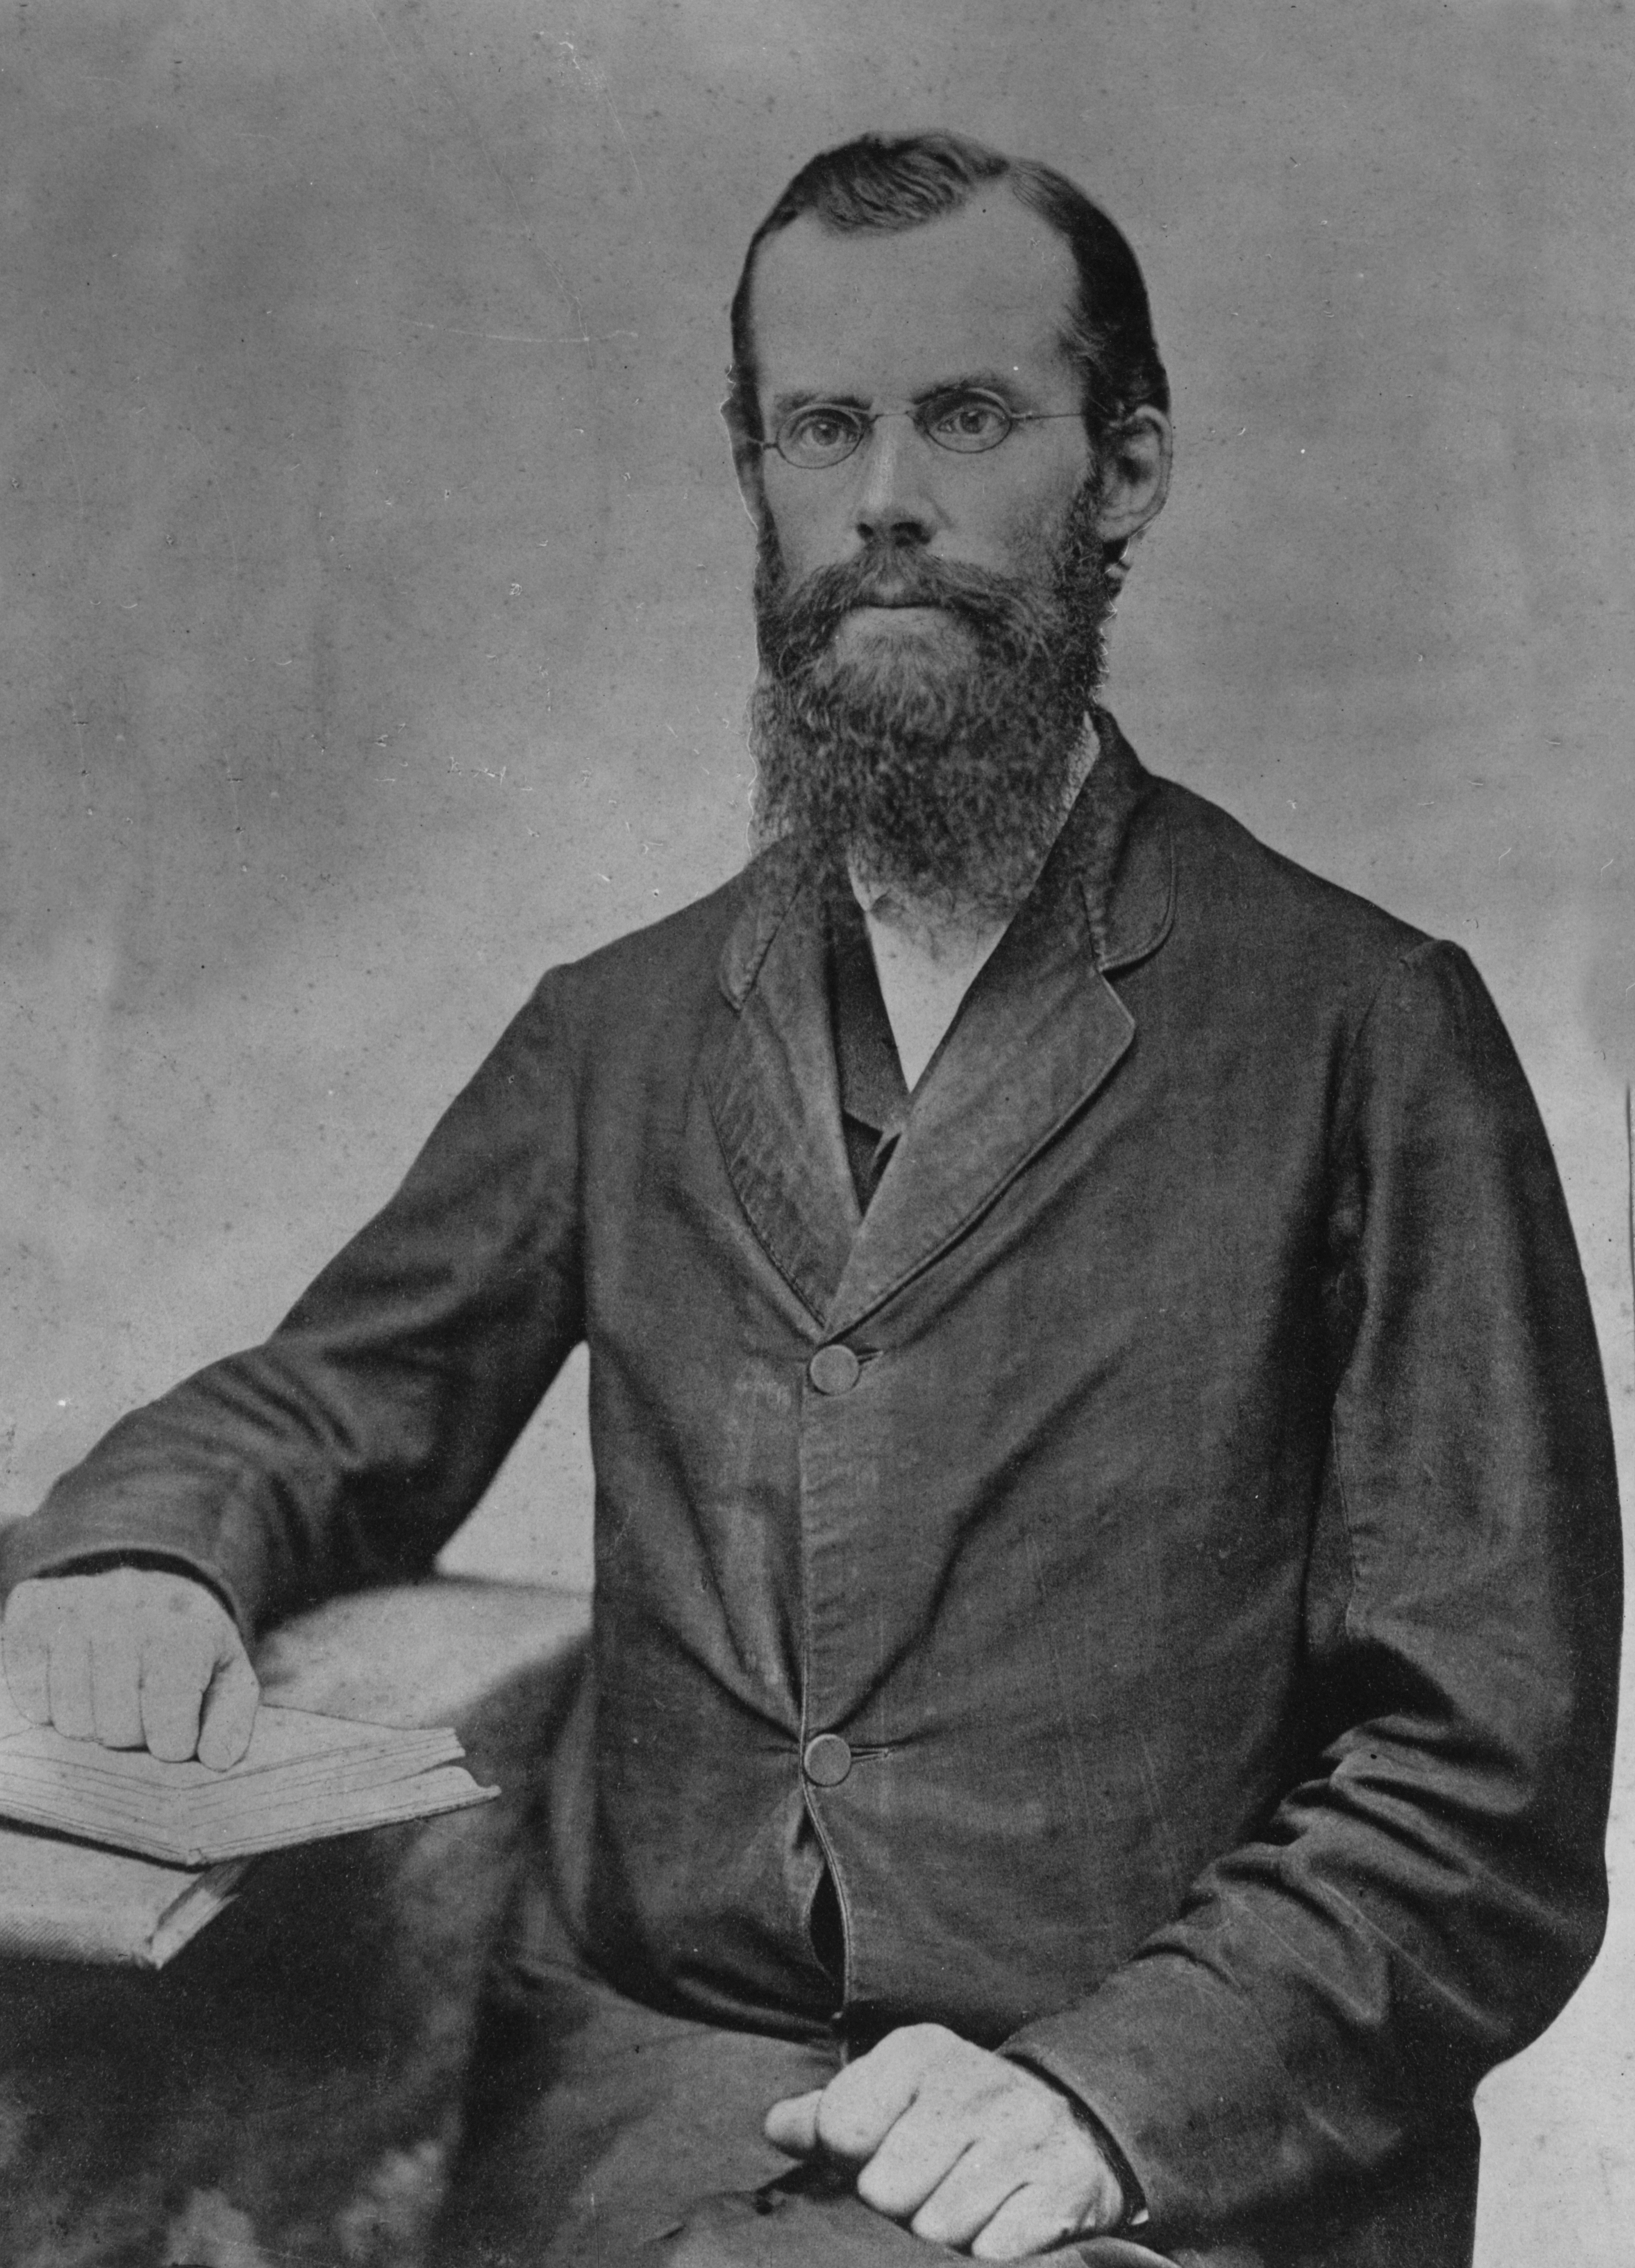
\includegraphics[width=1\linewidth]{images/john-nevins-andrews.jpg}
    \caption*{John Nevins Andrews (1829-1883)}
    \label{fig:j-n-andrews}
\end{figure}

J. N. Andrews powiedział: \others{\textbf{Doktryna o Trójcy, która została ustanowiona w Kościele przez sobór nicejski w 325 roku n.e.} \textbf{Ta doktryna \underline{niszczy osobowość Boga i Jego Syna Jezusa Chrystusa, naszego Pana}}...}[John. N. Andrews, The Advent Review and Sabbath Herald, 6 marca 1855, str. 185][http://documents.adventistarchives.org/Periodicals/RH/RH18550306-V06-24.pdf]

W kontekście trynitarnego rozumienia \emcap{osobowości Boga} można bezpiecznie powiedzieć, że \emcap{osobowość Boga}, czyli właściwość lub stan Boga jako osoby, w każdym rozumieniu doktryny o Trójcy jest tajemnicą. Problem polega na tym, że nie ma jasnego poglądu, kim jest ten \textit{jeden Bóg}, który jest osobą? Podstawowe twierdzenie mówi, że Bóg jest Jeden, ale Trzema, lub Jeden w Trzech; tak, Bóg jest osobą i jest jeden, ale jednocześnie jest trzema osobami. Ten pogląd nigdy nie może mieć jasnego postrzegania \emcap{osobowości Boga}. Ponadto zaprzeczy on najwyraźniejszemu świadectwu Pisma Świętego, że jedynym Bogiem jest Ojciec, a Chrystus jest prawdziwie Jego jednorodzonym Synem. Większość braci trynitarnych zgodziłaby się, że Chrystus jest realną i określoną istotą, ale gdyby trynitarianin miał zaakceptować Ojca jako realną i określoną Istotę, musiałby również zaakceptować Ducha Świętego jako realną i określoną istotę, tym samym zaprzeczając, że Duch Święty jest \textit{duchem}, środkiem, przez który Ojciec i Syn są wszechobecni. I odwrotnie, gdyby trynitarianin zaakceptował Ducha Świętego jako dosłownego ducha, niemającego ciała ani formy, zaprzeczyłby wtedy, że Ojciec jest realną, określoną istotą. W rozmowie o właściwości lub stanie Boga jako osoby nigdy nie ma jasnego poglądu na tę sprawę wśród zwolenników doktryny o Trójcy; to wybieg. \textit{«Wybiegi»} to słowo, którego Siostra White użyła do opisania oszustwa poprzez podstęp lub fortel w celu ukrycia, ucieczki lub uniknięcia\footnote{\href{https://www.merriam-webster.com/dictionary/subterfuges}{The Merriam-Webster, ‘subterfuges’} - “\textit{deception by artifice or stratagem in order to conceal, escape, or evade}”} prawdy; innymi słowy, coś, czego nie można złapać ani za głowę, ani za ogon. To jest główny powód, dla którego siostra White nie angażowała się w dyskusję o Trójcy, która miała się pojawić w Kościele Adwentystów Dnia Siódmego.

\egw{Ostrzeżono mnie, abym nie wchodziła w spór \textbf{dotyczący kwestii}, które \textbf{\underline{pojawią się}} w związku z \textbf{tymi sprawami, ponieważ spór \underline{mógłby doprowadzić ludzi do uciekania się do wybiegów, a ich umysły zostałyby odwiedzione od prawdy Słowa Bożego do przypuszczeń i domysłów}}. \textbf{Im więcej dyskutuje się o fantazyjnych teoriach, tym \underline{mniej ludzie będą wiedzieć o Bogu i o prawdzie, która uświęca duszę}}}[Lt232-1903.41; 1903][https://egwwritings.org/read?panels=p10197.50]

Kiedy czytamy dzieła pionierów Adwentystów Dnia Siódmego na temat \emcap{osobowości Boga}, widzimy, że nie wpadli oni w pułapkę Trójcy. Ich nietrynitarne poglądy na temat Boga nie wynikały z niewiedzy, lecz z poznania prawdy o \emcap{osobowości Boga}. Byli oni ludźmi o bystrym i szlachetnym intelekcie, rozumiejącymi cienką linię między prawdą a błędem. Ich zrozumienie \emcap{osobowości Boga} jest zrównoważone i solidne, mocno wsparte prostym i jasnym „\textit{tak mówi Pan}”.

Wielu adwentystów akceptuje dziś doktrynę o Trójcy, ponieważ Ellen White rzekomo ją zaakceptowała i promowała. Jest to dalekie od prawdy, a taki wniosek wynika z braku znajomości Ducha Proroctwa. Jeśli ktokolwiek był zaznajomiony z wierzeniami siostry White, to był to jej mąż James White. Oto co ma do powiedzenia o pismach swojej żony:

\others{\textbf{Zapraszamy wszystkich do porównania świadectw Ducha Świętego poprzez panią White ze słowem Bożym}. \textbf{I w tym nie zapraszamy was do porównywania ich \underline{z waszym wyznaniem wiary}}. To jest zupełnie co innego. \textbf{\underline{Trynitarianin może porównać je ze swoim wyznaniem wiary i potępić je, ponieważ się z nim nie zgadzają}}. Przestrzegający niedzieli lub człowiek, który uważa wieczne męki za ważną prawdę, i pastor, który kropi niemowlęta, każdy może potępić świadectwa pani White, ponieważ nie zgadzają się z ich szczególnymi poglądami. I setka innych, z których każdy ma inne poglądy, może dojść do tego samego wniosku. \textbf{Jednak ich autentyczność nigdy nie może być sprawdzona w ten sposób}.}[James S. White, The Advent Review, and Herald of the Sabbath, 13 czerwca 1871.][https://documents.adventistarchives.org/Periodicals/RH/RH18710613-V37-26.pdf]

James White był najbliższym współpracownikiem Ellen White, osobą, która była z nią jedno w Bożym budowaniu Kościoła Adwentystów Dnia Siódmego. Mamy jasne i bezpośrednie świadectwo od niego, że pisma Ellen White nie są trynitarne. Dziś uczeni przedstawiają fałszywą narrację, że Ellen White rozwinęła swoje zrozumienie doktryny o Trójcy i ostatecznie ją zaakceptowała i głosiła. Ale widzimy, że Ellen White nie zmieniła swojego stanowiska w sprawie \emcap{osobowości Boga} ani nie przyjęła doktryny o Trójcy. Była jednoznaczna w swoim twierdzeniu, że nigdy tego nie zrobiła. Kiedy nadszedł kryzys Kellogga dotyczący \emcap{osobowości Boga}, pozostała niewzruszona w swoim poglądzie, tak jak wszyscy wcześni pionierzy Adwentystów Dnia Siódmego — a jej postępowanie z dr. Kelloggiem to udowadnia. To prawda, doktryna o Trójcy \textit{nie może być przyjęta przez lojalnych wobec wiary i zasad, które wytrzymały wszelki sprzeciw szatańskich wpływów}.\footnote{\egw{Łatane teorie nie mogą być przyjęte przez lojalnych wobec wiary i zasad, które wytrzymały wszelki sprzeciw szatańskich wpływów}[Lt253-1903.28; 1903][https://egwwritings.org/read?panels=p14068.9980036]} Dzisiejsza oficjalna narracja, że Ellen White nauczała o Trójcy, przypomina twierdzenie dr. Kellogga, że książka \textit{The Living Temple} nauczała tego samego, co Ellen White. \egwinline{\textbf{Ale broń Boże, żeby ten pogląd przeważył}}[SpTB02 53.3; 1904][https://egwwritings.org/read?panels=p417.272]

% Pionierzy adwentyzmu i doktryna o Trójcy

\begin{titledpoem}
    \stanza{
        Loughborough pytany o Trójcy zastrzeżenia, \\
        Trzy powody podał godne rozważenia. \\
        Sprzeczna ze zdrowym rozsądkiem i z Pismem całym, \\
        Z pogańskich źródeł pochodzi z blaskiem niemałym.
    }

    \stanza{
        Jak może Bóg być trzema i jednym zarazem? \\
        Jak może modlić się do siebie własnym głosem? \\
        Jan siedemnasty rozdział tę doktrynę obala, \\
        Gdy Chrystus o Ojcu jako odrębnym wspomina.
    }

    \stanza{
        Pionierzy widzieli jasno, co Pismo objawia, \\
        Że Ojciec jest Bogiem, a Chrystus Synem zostaje. \\
        Nie przez tajemnicę, lecz przez proste słowa, \\
        Prawda o Bogu w ich pismach się chowa.
    }

    \stanza{
        Ellen White z mężem w jedności trwali, \\
        Tę samą prawdę o Bogu wyznawali. \\
        Nie zmieniła poglądów, jak niektórzy twierdzą, \\
        Lecz wierną pozostała prawdzie z Bożą pieczęcią.
    }
\end{titledpoem}

